\appendix
\chapter{Appendix}
\subsection{The reversed shader}\label{apx:shader}
\begin{lstlisting}
Shader "InsideVisible" {
Properties{
_MainTex("Base (RGB)", 2D) = "white" {}
}
SubShader{
	Tags { "RenderType" = "Opaque" }
	Cull front    // ADDED BY BERNIE, TO FLIP THE SURFACES
	LOD 100

	Pass {
		CGPROGRAM
			#pragma vertex vert
			#pragma fragment frag

			#include "UnityCG.cginc"

			struct appdata_t {
				float4 vertex : POSITION;
				float2 texcoord : TEXCOORD0;
			};

			struct v2f {
				float4 vertex : SV_POSITION;
				half2 texcoord : TEXCOORD0;
			};

			sampler2D _MainTex;
			float4 _MainTex_ST;

			v2f vert(appdata_t v)
			{
				v2f o;
				o.vertex = UnityObjectToClipPos(v.vertex);
				// ADDED BY BERNIE:
				v.texcoord.x = 1 - v.texcoord.x;
				o.texcoord = TRANSFORM_TEX(v.texcoord, _MainTex);
				return o;
			}

			fixed4 frag(v2f i) : SV_Target
			{
				fixed4 col = tex2D(_MainTex, i.texcoord);
				return col;
			}
		ENDCG
	}
	}

}
\end{lstlisting}
\subsection{Keras performance table}
\begin{figure}[H]
	\centering        
	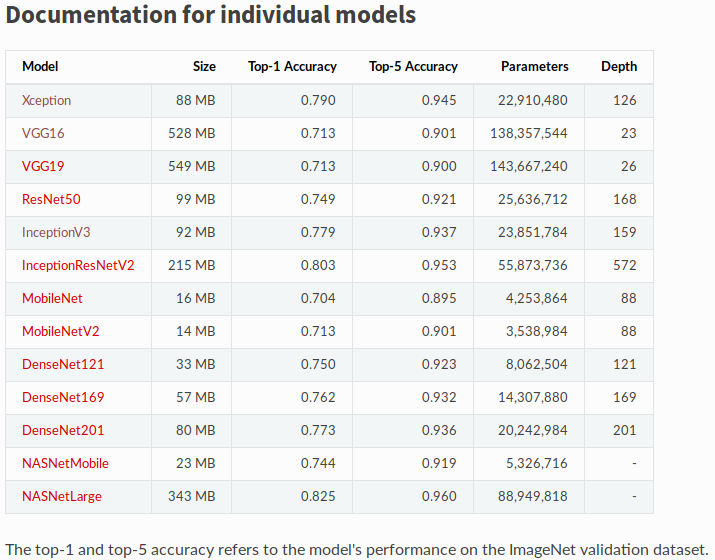
\includegraphics[width=0.75\textwidth]{project/images/KerasModels.png}
	\caption{Keras individual models performance}
	\label{fig:keras}
\end{figure}
\subsection{R-Pi Testing Code}
\begin{lstlisting}
# GPIO management
import RPi.GPIO as GPIO
# Serial communication
import time
import zmq
# sigint capture
import signal

# Setting up GPIO ports for LED
GPIO.setmode(GPIO.BCM)
GPIO.setwarnings(False)
GPIO.setup(18,GPIO.OUT)
GPIO.setup(23,GPIO.OUT)
GPIO.setup(24,GPIO.OUT)
GPIO.setup(25,GPIO.OUT)

# Set up context for communication
context = zmq.Context()
socket = context.socket(zmq.REP)
socket.bind("tcp://*:9999")

def signal_handler(sig, frame):
    print("Gracefull Exit")
    GPIO.output(18,GPIO.LOW)
    GPIO.output(23,GPIO.LOW)
    GPIO.output(24,GPIO.LOW)
    GPIO.output(25,GPIO.LOW)
    # socket.send(b"Interupt")
    sys.exit(0)
# Infinite loop
while True:
    signal.signal(signal.SIGINT, signal_handler)
    # Wait for request from client
    message = socket.recv()
    # print("Status movement: %s" % message)
    # print "Forward is On"
    if(message == "Forward"):
        GPIO.output(18,GPIO.HIGH)
    elif(message == "Left"):
        GPIO.output(23,GPIO.HIGH)
    elif(message == "Right"):
        GPIO.output(24,GPIO.HIGH)
    elif(message == "Backward"):
        GPIO.output(25,GPIO.HIGH)
    else:
        # print "Forward is Off"
        GPIO.output(18,GPIO.LOW)
        GPIO.output(23,GPIO.LOW)
        GPIO.output(24,GPIO.LOW)
        GPIO.output(25,GPIO.LOW)
    time.sleep(0.1)
    socket.send(b"SoFarGood")
\end{lstlisting}